\documentclass[11pt, letterpaper, onecolumn]{article}

% Imports
\usepackage[english]{babel}
\usepackage{fancyhdr}
\usepackage{extramarks}
\usepackage{amsmath, amsthm, amsfonts,mathtools, framed}
\usepackage[shortcuts]{extdash} % Use \-/ for hyphenated words
\usepackage{environ}
\usepackage{fancyvrb}
\usepackage[top=1.00in, bottom=1.00in, left=0.75in, right=0.75in]{geometry}
\usepackage{algorithm}
\usepackage{algpseudocode}
\usepackage{accents}
% Pseudocode enabler
\usepackage{listings}
\usepackage{color}

\usepackage{pdfpages}

\definecolor{dkgreen}{rgb}{0,0.6,0}
\definecolor{gray}{rgb}{0.5,0.5,0.5}
\definecolor{mauve}{rgb}{0.58,0,0.82}

\lstset{frame=tb,
  language=Java,
  aboveskip=3mm,
  belowskip=3mm,
  showstringspaces=false,
  columns=flexible,
  basicstyle={\small\ttfamily},
  numbers=none,
  numberstyle=\tiny\color{gray},
  keywordstyle=\color{blue},
  commentstyle=\color{dkgreen},
  stringstyle=\color{mauve},
  breaklines=true,
  breakatwhitespace=true,
  tabsize=3
}

% tikz
\usepackage{pgf}
\usepackage{tikz}
\usetikzlibrary{arrows,automata}

% Page
\headsep=0.3in
\linespread{1.15}
\setlength\parindent{0pt}

% Horizontal Rules
\newcommand{\hwRuleWidth}{0.4pt}
\renewcommand\headrulewidth{\hwRuleWidth}
\renewcommand\footrulewidth{\hwRuleWidth}

% Header and Footer
\pagestyle{fancy}
\lhead{\hwAuthor\ (\hwSection)}
\chead{\hwClass\ (\hwInstructor): \hwTitle}
\rhead{\firstxmark}
\lfoot{\lastxmark}
\cfoot{\thepage}
\newcommand{\enterProblemHeader}[2]{
  \nobreak\extramarks{}{Problem \arabic{#1}.\arabic{#2} continued on next page\ldots}\nobreak{}
  \nobreak\extramarks{Problem \arabic{#1}.\arabic{#2} (continued)}{Problem \arabic{#1}.\arabic{#2} continued on next page\ldots}\nobreak{}
}
\newcommand{\exitProblemHeader}[2]{
  \nobreak\extramarks{Problem \arabic{#1}.\arabic{#2} (continued)}{Problem \arabic{#1}.\arabic{#2} continued on next page\ldots}\nobreak{}
  \nobreak\extramarks{Problem \arabic{#1}.\arabic{#2}}{}\nobreak{}
}

% Counters
\setcounter{secnumdepth}{0}
\newcounter{partCounter}
\setcounter{partCounter}{1}
\newcounter{hwProblemCounter}
\newcounter{hwSubProblemCounter}
\numberwithin{equation}{hwProblemCounter}
\numberwithin{figure}{hwProblemCounter}

% Environments
\newenvironment{problem}[3] {
  \setcounter{hwProblemCounter}{#2}
  \setcounter{hwSubProblemCounter}{#3}
  \setcounter{partCounter}{1}
  \enterProblemHeader{hwProblemCounter}{hwSubProblemCounter}

  \large{\textbf{Problem #2.#3: #1}}\\
}{
  \exitProblemHeader{hwProblemCounter}{hwSubProblemCounter}
}

\newcommand{\question}[2]{\textbf{(#1)\ }\ #2\\}

\newenvironment{Proof}[1][Proof]
  {\proof[#1]\leftskip=1cm\rightskip=1cm}
  {\endproof}
%-------------------------------------------------------------------------------
% Assignmnet Variables
%-------------------------------------------------------------------------------
\newcommand{\hwTitle}{Homework 1}
\newcommand{\hwDueDate}{April 19, 2017}
\newcommand{\hwClass}{CS 181}
\newcommand{\hwInstructor}{Nicolas Christou}
\newcommand{\hwAuthor}{Earle Aguilar}
\newcommand{\hwSection}{804501476}
% First Problem
\setcounter{hwProblemCounter}{1}
\setcounter{hwSubProblemCounter}{0}

%-------------------------------------------------------------------------------
\begin{document}
%-------------------------------------------------------------------------------
% TITLE
%-------------------------------------------------------------------------------
{\centering
  \Large{\textbf{\hwTitle}}\\
  \vspace{0.1in}\normalsize{\hwDueDate}\\
  \vspace{0.1in}\textbf{\hwAuthor} (\hwSection)\\
  \vspace{0.1in}\rule{\textwidth}{\hwRuleWidth}}\\


\newcommand{\msum}{\displaystyle \sum}
\newcommand{\betah}{\hat{\beta}}
\newcommand{\pmatb}{\begin{pmatrix}}
\newcommand{\pmate}{\end{pmatrix}}
%-------------------------------------------------------------------------------
% Problem 1.0
%------------------------------------------------------------------------------

\begin{problem}{}{1}{0}
  \begin{align}
    SSE &= \msum_{i=1}^n e_i^2 = (Y-X\beta)^{'}(Y-X\beta) \\
        &= Y^{'}Y - Y^{'}X \betah - \betah^{'}X^{'}Y + \betah^{'}X^{'}X\betah \\
  \end{align}
  
  Substitude $\betah = (X^{'}X)^{-1}X^{'}Y$ to the last term

  \begin{align}
    SSE &= Y^{'}Y-Y^{'}X\betah -\betah^{'}X^{'}Y+\betah^{'}X^{'}X((X^{'}X)^{-1}X^{'}Y) \\
        &= Y^{'}Y-Y^{'}X\betah -\betah^{'}X^{'}Y + \betah^{'}X^{'}Y \\
    \Aboxed{SSE &= Y^{'}Y-\betah^{'}X^{'}Y}
  \end{align}
  
  \begin{align}
    SSE &= Y^{'}Y-Y^{'}X\betah -\betah^{'}X^{'}Y+\betah^{'}X^{'}X((X^{'}X)^{-1}X^{'}Y) \\
        &= Y^{'}Y-Y^{'}X\betah -\betah^{'}X^{'}Y + \betah^{'}X^{'}HY \\
    \Aboxed{SSE &= Y^{'}Y-\betah^{'}X^{'}\hat{Y}}
  \end{align}
  
  \begin{align}
    SSE &= Y^{'}Y-Y^{'}X\betah -\betah^{'}X^{'}Y+\betah^{'}X^{'}X((X^{'}X)^{-1}X^{'}Y) \\
        &= Y^{'}Y-Y^{'}X\betah -\betah^{'}X^{'}Y + \betah^{'}X^{'}Y \\
    SSE &= Y^{'}Y-\betah^{'}X^{'}Y
  \end{align}
  Substitude normal equations $X^{'}Y=X^{'}X\betah$ \\
    \begin{align}
    SSE &= Y^{'}Y-Y^{'}X\betah -\betah^{'}X^{'}Y+\betah^{'}X^{'}X((X^{'}X)^{-1}X^{'}Y) \\
        &= Y^{'}Y-Y^{'}X\betah -\betah^{'}X^{'}Y + \betah^{'}X^{'}Y \\
    \Aboxed{SSE &= Y^{'}Y-\betah^{'}X^{'}X\betah}
  \end{align}
\end{problem}
%-------------------------------------------------------------------------------
% Problem 2.0
%-------------------------------------------------------------------------------
\begin{problem}{}{2}{0}
  \begin{align}
    X &=
    \begin{pmatrix} 
      1         &x_{11}&x_{12}&\cdots&.001x_{1i}&\cdots&x_{1k}\\
      1         &x_{21}&x_{22}&\cdots&.001x_{2i}&\cdots&x_{2k}\\
      \vdots    &\vdots&\vdots&\ddots&\vdots    &      &\vdots\\
      1         &x_{i1}&x_{i2}&\cdots&.001x_{ii}&\cdots&x_{ik}\\
      \vdots    &\vdots&\vdots&      &\vdots    &\ddots&\vdots\\
      1         &x_{n1}&x_{n2}&\cdots&.001x_{ni}&\cdots&x_{nk} 
    \end{pmatrix}
\end{align}

\begin{align}
  X^{'}X &=
      \begin{pmatrix}  
        n                 &\sum x_{i1}               &\sum x_{i2}               &\cdots&.001\sum\sum x_{ji}        &\cdots&\sum x_{ik}\\
        \sum x_{i1}        &\sum x_{i1}^2             &\sum x_{i1}x_{i2}          &\cdots&.001\sum x_{i1} \sum x_{ji} &\cdots&\sum x_{i1} x_{ik} \\
        \sum x_{i2}        &\sum x_{i1}x_{i2}          &\sum x_{i2}^2             &\cdots&.001\sum x_{i2}\sum x_{ji}  &      &\sum x_{i2} x_{ik} \\
        \vdots            &\vdots                   &\vdots                   &\ddots&\vdots                    &       &\vdots\\
        .001\sum\sum x_{ji}&.001\sum x_{i1}\sum x_{ji} &.001\sum x_{i2}\sum x_{ji}&\cdots&(.001)^2\sum x_{ii}^2       &\cdots&.001\sum x_{ik} x_{ji} \\
        \vdots            &\vdots                   &\vdots                   &      &\vdots                    &\ddots&\vdots\\
        \sum x_{ik}        &\sum x_{i1}x_{ik}          &\sum x_{i1}x_{ik}         &\cdots&.001\sum x_{ik} x_{ji}      &\cdots&\sum x_{ik}^2 
      \end{pmatrix}
\end{align}

\begin{align}
  \betah_i &= ((.001)^2X_{ii}^{'} X_{ii})^{-1}(.001X_{ii}^{'})Y \\
  \betah_i &= 1000 (X_{ii}^{'} X_{ii})^{-1}X_{ii}^{'}Y \\
           &= 1000 \betah_i
\end{align}
\end{problem}

%-------------------------------------------------------------------------------
% Problem 3.0
%-------------------------------------------------------------------------------
\begin{problem}{}{3}{0}
  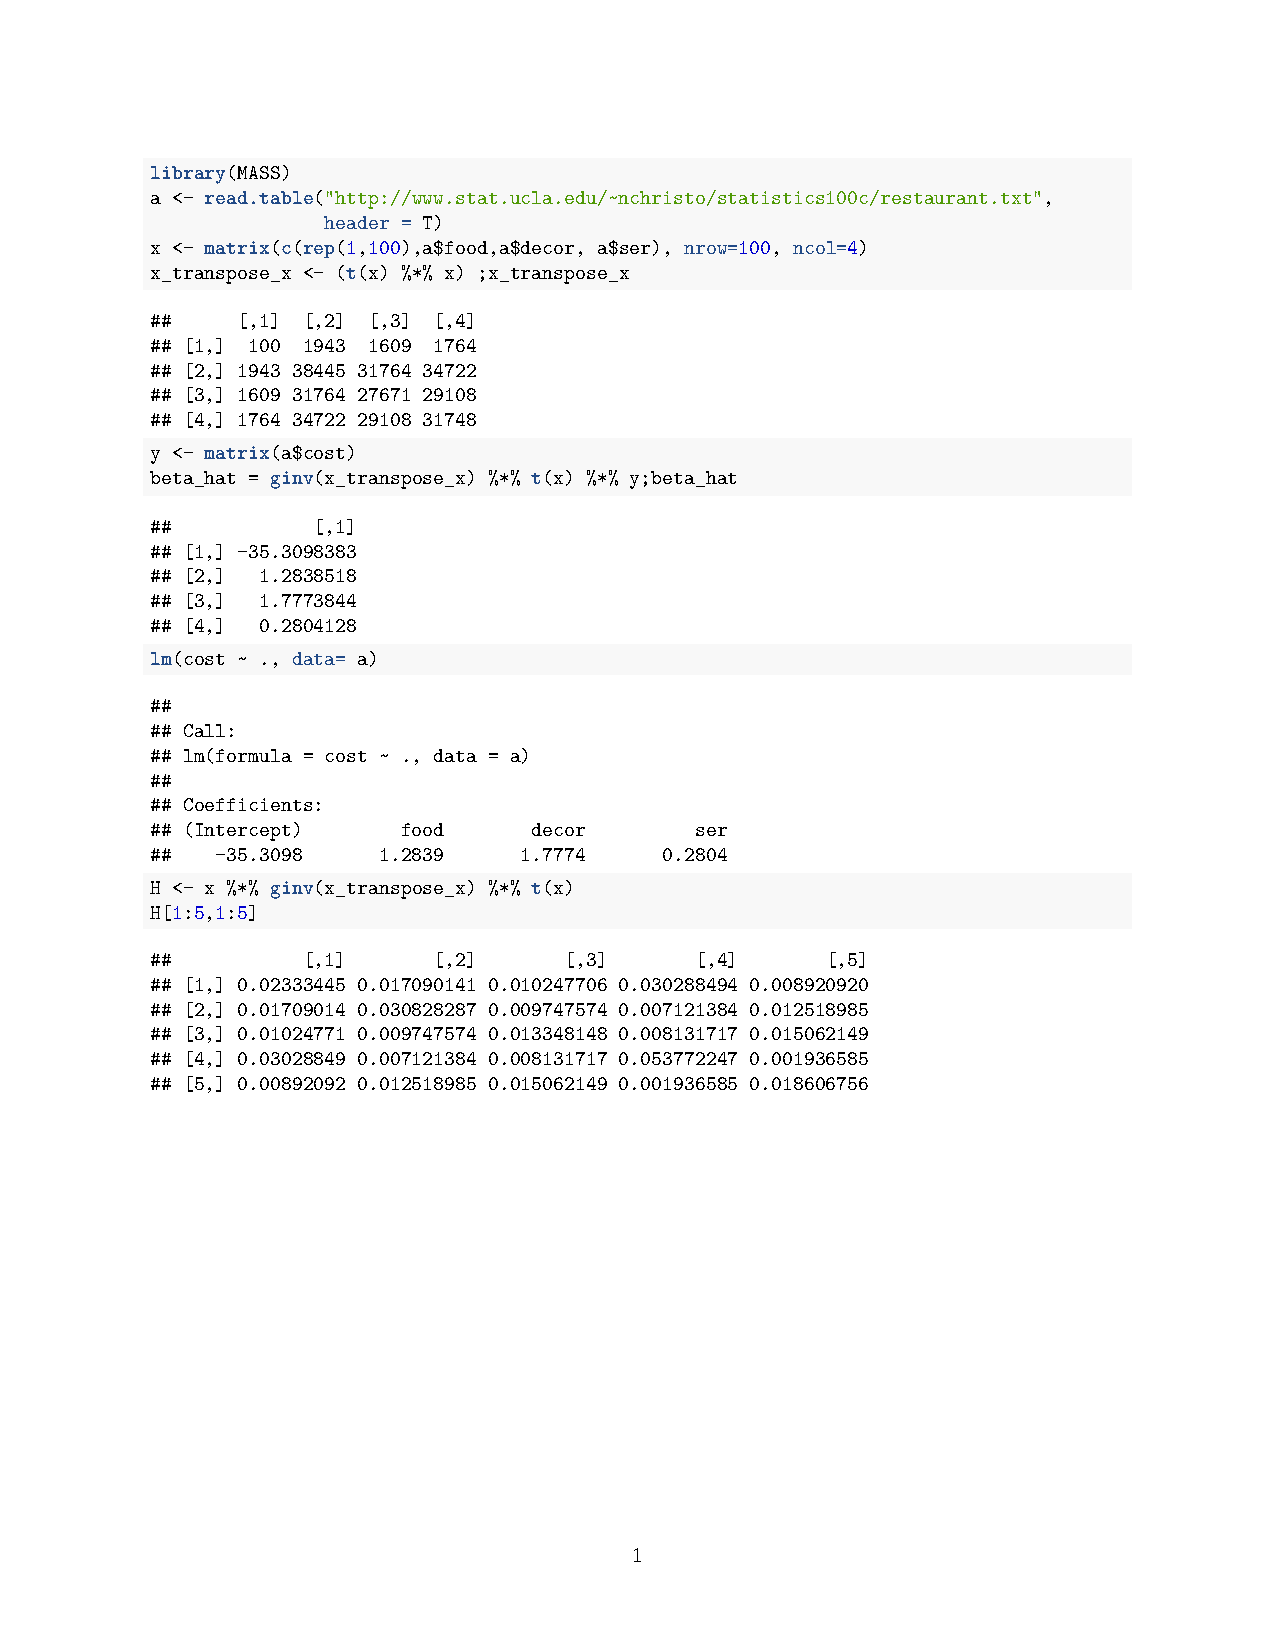
\includegraphics[scale=0.90]{prob2.pdf}
\end{problem}
%-------------------------------------------------------------------------------
% Problem 4.0
%-------------------------------------------------------------------------------
\begin{problem}{}{4}{0}
  {\tiny
    \setlength{\abovedisplayskip}{6pt}
    \setlength{\belowdisplayskip}{\abovedisplayskip}
    \setlength{\abovedisplayshortskip}{0pt}
    \setlength{\belowdisplayshortskip}{3pt}
    \begin{align}
      (Y-X\betah+X\betah-X\beta)^{'}(Y-X\betah+X\betah-X\beta) \\
      ((Y-X\betah)+X(\betah-\beta))^{'}((Y-X\betah)+X(\betah-\beta)) \\
      (Y-X\betah)^{'}(Y-X\betah) + (Y-X\betah)^{'}X(\betah-\beta) +
      (\betah-\beta)^{'}X^{'}(Y-X\betah) + (\betah-\beta)^{'} X^{'} X(\betah-\beta) \\   
      (Y-X\betah)^{'}(Y-X\betah) + (Y-\hat{Y})^{'}X(\betah-\beta) +
      (\betah-\beta)^{'}X^{'}(Y-\hat{Y}) + (\betah-\beta)^{'} X^{'} X(\betah-\beta) \\
      (Y-X\betah)^{'}(Y-X\betah) + (\betah-\beta)^{'} X^{'} X(\betah-\beta) 
    \end{align}
  }%
\end{problem}
% -------------------------------------------------------------------------------
% Problem 5.0
%-------------------------------------------------------------------------------
\begin{problem}{}{5}{0}
  \begin{align}
    E[\hat{Y}^{'}\hat{Y}] &= E [(HY)^{'}HY] = E[Y^{'}H^{'}HY] \\
    &= E[tr(Y^{'}HY)] = tr(HE[Y^{'}Y]) \\
    &= tr(H(\sigma^2 I + X\beta \beta^{'}X^{'})) = tr(\sigma^2 H + X\beta \beta^{'}X^{'}) \\
    &= tr(\sigma^2H) + tr(X\beta \beta^{'}X^{'}) \\
    E[\hat{Y}^{'}\hat{Y}] &= \sigma(K+1) + \beta^{'}X^{'}X\beta
  \end{align}
\end{problem}
%-------------------------------------------------------------------------------
% Problem 6.0
%-------------------------------------------------------------------------------
\begin{problem}{}{6}{0}
  \begin{align}
    Q &= \begin{pmatrix} 
      \betah_1 -2\betah_2+3\betah_4 \\
      \betah_0 + \betah_4 + 3 \betah_5 
    \end{pmatrix} \\
      &=   
        \begin{pmatrix}
          0 & 1 & -2 & 0 & 3 & 0 \\
          1 & 0 & 0  & 0 & 1 & 3
        \end{pmatrix}   
        \begin{pmatrix}
          \betah_0 \\
          \betah_1 \\
          \betah_2 \\
          \betah_3 \\
          \betah_4 \\
          \betah_5 \\
        \end{pmatrix} \\
    Q &=c\betah
  \end{align}
We know that $\betah \sim N_6(\beta, \sigma (X^{'}X)^{-1})$ then,
\begin{align}
  E[Q] &= E[c\betah] = c E[\betah] \\
  E[Q] &= c\beta \\
  Var(Q) &= Var(c\betah) \\
  Var(Q) &= c(\sigma (X^{'}X)^{-1})c^{'}
\end{align}
\begin{align}
  \Aboxed{Q \sim N_2(c\beta,  \sigma c(X^{'}X)^{-1}c^{'})}
\end{align}
\end{problem}
\newpage
%-------------------------------------------------------------------------------
% Problem 7.0
%-------------------------------------------------------------------------------
\begin{problem}{}{7}{0}
\section{a}
\begin{align}
  \betah_1 = (X_1^{'}X_1)^{-1}X_1^{'}Y_1 \\
  \betah_2 = (X_2^{'}X_2)^{-1}X_2^{'}Y_2 
\end{align}
\section{b}
\begin{align}
  \betah &= \bigg( \pmatb X_1^{'}&X_2^{'} \pmate \pmatb X_1 \\ X_2 \pmate \bigg)^{-1}
  \pmatb X_1^{'}&X_2^{'} \pmate \pmatb Y_1 \\ Y_2 \pmate \\
         &= \pmatb X_1^{'}X_1 + X_2^{'}X_2 \pmate^{-1} 
           \pmatb X_1^{'}&X_2^{'} \pmate \pmatb Y_1 \\ Y_2 \pmate \\
  \betah &= \pmatb X_1^{'}X_1 + X_2^{'}X_2 \pmate^{-1}
           \pmatb X_1^{'}Y_1 + X_2^{'}Y_2 \pmate
\end{align}
\section{c}
\begin{align}
  \betah &= (2X_1^{'}X_1)^{-1}(X_1^{'}Y_1 + X_2^{'}Y_2) \\
  &= \frac{1}{2}(X_1^{'}X_1)^{-1}(X_1^{'}Y_1 + X_2^{'}Y_2) \\
  &= \frac{1}{2}[(X_1^{'}X_1)^{-1}X_1^{'}Y_1 + (X_1^{'}X_1)^{-1}X_2^{'}Y_2] \\
  &= \frac{1}{2}[(X_1^{'}X_1)^{-1}X_1^{'}Y_1 + (X_2^{'}X_2)^{-1}X_2^{'}Y_2] \\
  \betah &= \frac{1}{2}(\betah_1 + \betah_2)
\end{align}
\end{problem}
\end{document}


 
% \begin{align}
% \end{align}
% \frac{}{}
